\documentclass{beamer}

\mode<presentation>
\usetheme[hideothersubsections]{PaloAlto}
\usecolortheme{seagull}
\usefonttheme{serif}
\pgfdeclareimage[height=1cm]{uni}{HWU_logo}
\logo{\pgfuseimage{uni}}

\setbeamertemplate{caption}[numbered]

\usepackage{hyperref}
\usepackage{cleveref}
\usepackage{listings}

\lstset{basicstyle=\selectfont\ttfamily\color{white},
  showstringspaces=false,
  commentstyle=\color{red},
  keywordstyle=\color{blue},
  backgroundcolor=\color{black},
  frame={single}
}

\title{Introduction to \LaTeX}
\author[OTB \& LF]{Oliver T. Brown \& Liam Fitzgerald}
\institute[HWU]{Heriot-Watt University}
\date[2016-01-26]{26th January 2016}

\begin{document}

\begin{frame}
	\titlepage
\end{frame}

\section{Outline}
\begin{frame}
	\frametitle{Outline}
	\tableofcontents
\end{frame}

\section{What is \LaTeX?}

\subsection[LayTECH]{Pronunciation}
\begin{frame}
\frametitle{What is \LaTeX?}
\framesubtitle{Pronunciation}
\uncover<1->{Every single `Intro to \LaTeX' presentation begins this way...} \vspace{\baselineskip}

\uncover<2->{It is pronounced Lay-tech/Lay-teck, \alert{NOT} Lay-tecks.} \vspace{\baselineskip}

\uncover<3->{(Sometimes Lah-tech/Lah-teck)} \vspace{\baselineskip}

\uncover<4->{(Never Lah-tecks)}
\end{frame}

\subsection{Typesetting Language}
\begin{frame}
\frametitle{What is \LaTeX?}
\framesubtitle{Typesetting Language}
\begin{itemize}
\item Builds on the TeX typesetting program developed in a time before graphical interfaces, the 1970s, by Donald E Knuth.
\item It is a \emph{typesetting language}, not a word-processor (more on that shortly).
\item Designed so that the author's job is just to specify the kind of document they want, and produce the content.
\item In principle a nicely presented document can be produced without the author having ever seen it. Useful on a command line computer system!
\end{itemize}
\end{frame}

\subsection{Not Word}
\begin{frame}
\frametitle{What is \LaTeX?}
\framesubtitle{Not Word}
\emph{All right, but basically it's for writing documents, so why is it different from [MY FAVOURITE WORD PROCESSING SOFTWARE]?}
\vspace{\baselineskip}
\begin{itemize}
\item You use commands to define the style of the document.
\item The document is then \emph{compiled}.
\item You don't get to see what it will look like until it has compiled.
\item You don't necessarily get all that much choice about what it looks like.
\end{itemize}
\end{frame}

\section{How does it work?}

\subsection{Obtaining \LaTeX}
\begin{frame}
\frametitle{How does it work?}
\framesubtitle{Obtaining \LaTeX}
\begin{itemize}
\item \alert{Hold on.} There's a pretty good chance if you're using a uni computer, any kind of linux machine, or you've installed a \LaTeX\ IDE that you already have it installed!
\item Having multiple TeX distributions installed can quite messy, so it's definitely worth checking.
\item If you definitely don't then the easiest way is probably to download the TeX Live package from \url{http://www.tug.org/texlive/} -- be warned, the download can take some time...
\item More information on obtaining TeX and \LaTeX can be found at \url{https://latex-project.org/ftp.html}.
\end{itemize}
\end{frame}

\subsection{Compilation}

\lstset{language=bash}

\begin{frame}[fragile]
\frametitle{How does it work?}
\framesubtitle{Compilation}

Back in the good old days you may have had to enter a command sequence like one of the following...

\begin{lstlisting}[caption={Command sequence for this presentation.}, label={lst:1}]
>> pdflatex intro_latex.tex
>> pdflatex intro_latex.tex
>> evince intro_latex.tex
\end{lstlisting}

\begin{lstlisting}[caption={Command sequence for a document containing BibTeX references.}, label={lst:2}]
>> pdflatex OTB_phdthesis_v00.tex
>> bibtex OTB_phdthesis_v00.tex
>> pdflatex OTB_phdthesis_v00.tex
>> pdflatex OTB_phdthesis_v00.tex
>> evince OTB_phdthesis_v00.tex
\end{lstlisting}

\end{frame}

\begin{frame}
\frametitle{How does it work?}
\framesubtitle{Compilation}

In these more enlightened times you'll almost certainly be using an IDE to write and compile your document, so you probably just have to click the `build' button. As an example, \cref{fig:1} below shows a screenshot of TeXMaker, which I used to create this presentation. You can see it has a `Quick Build' button right at the top, as well as a `View PDF' button. 

\begin{figure}[h!]
\centering
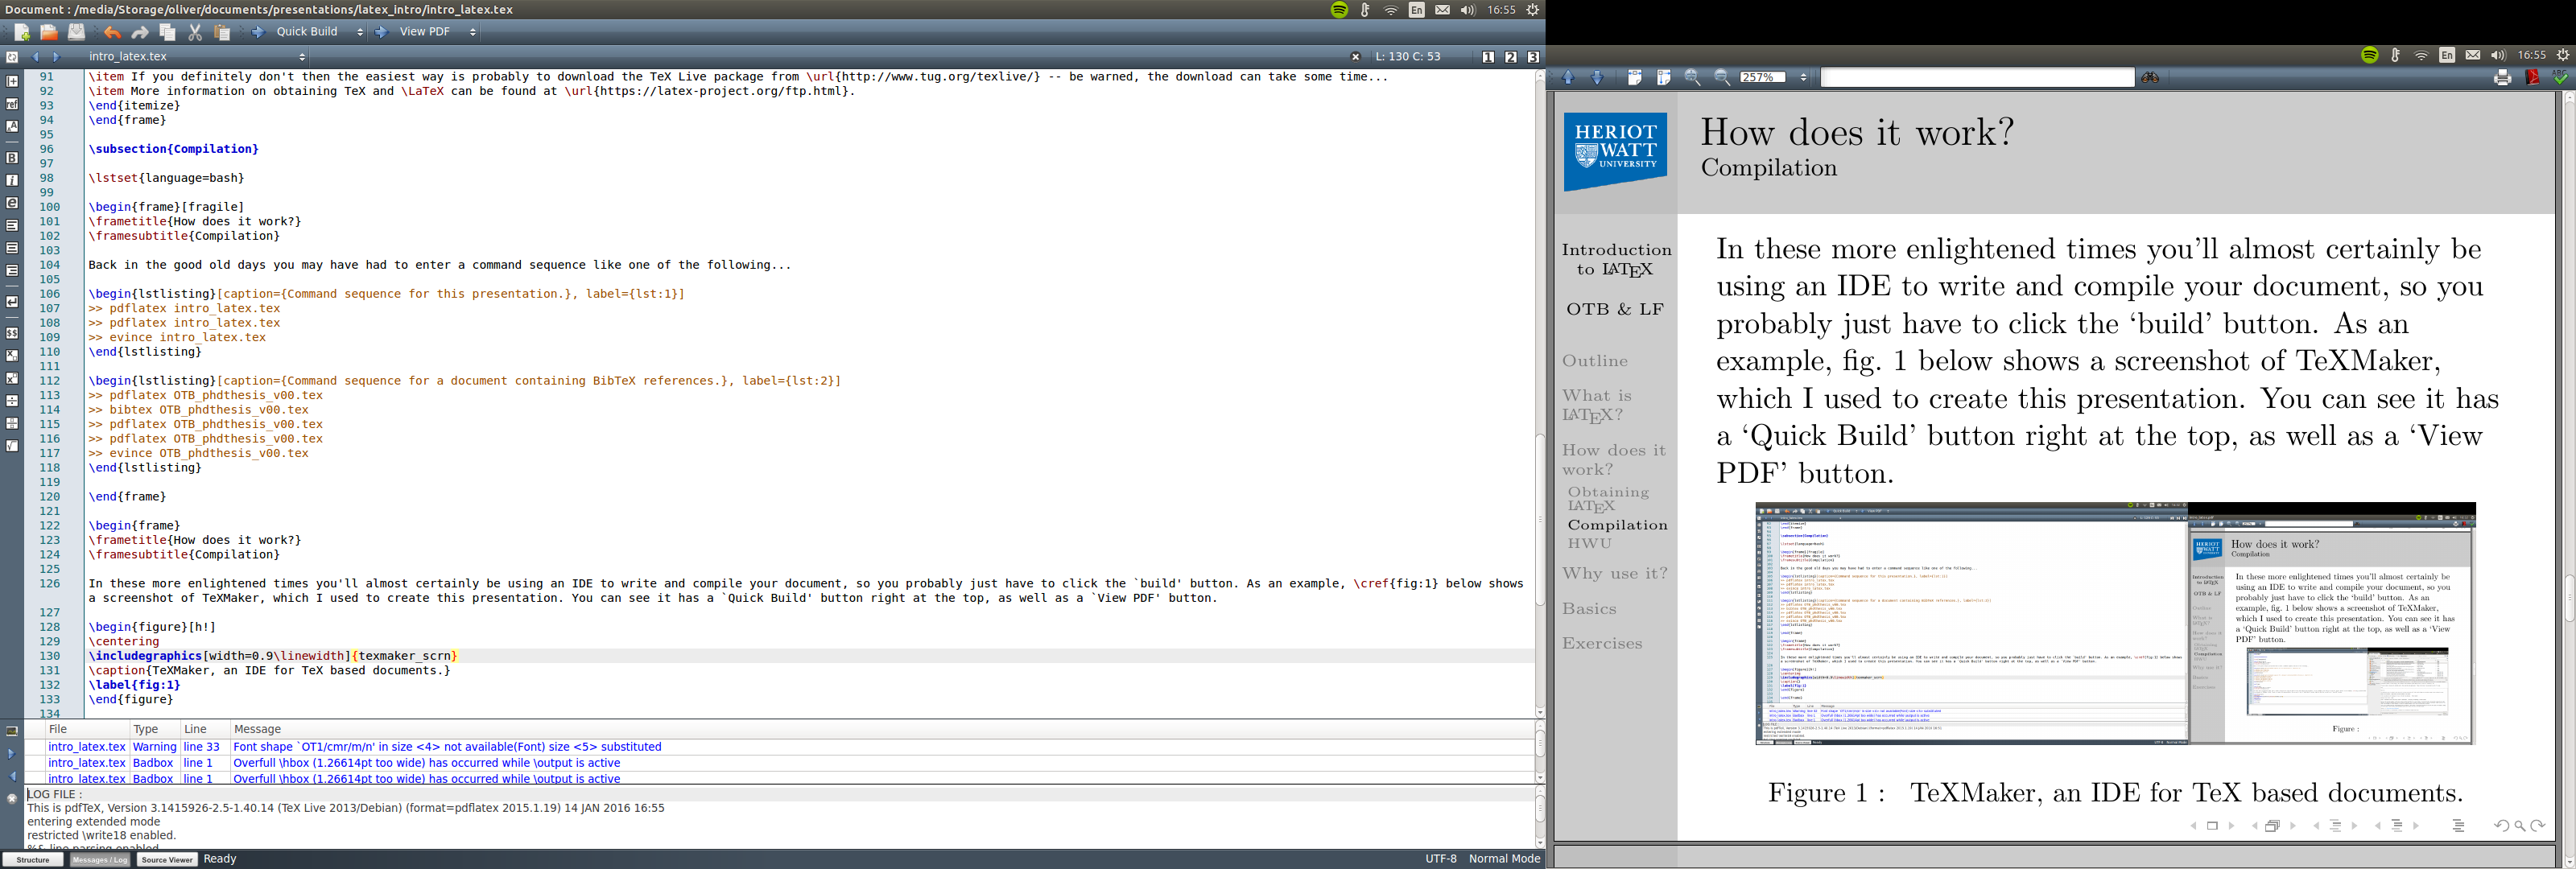
\includegraphics[width=0.9\linewidth]{texmaker_scrn}
\caption{TeXMaker, an IDE for TeX based documents.}
\label{fig:1}
\end{figure}

\end{frame}

\subsection[HWU]{Using \LaTeX at Heriot-Watt}
\begin{frame}
\end{frame}

\section{Why use it?}

\subsection[Cons]{Disadvantages}
\begin{frame}
\end{frame}

\subsection[Pros]{Advantages}
\begin{frame}
\end{frame}

\section{Basics}
\begin{frame}
\end{frame}

\section{Exercises}
\begin{frame}
\end{frame}

\end{document}